\documentclass[12pt, letterpaper]{article}

\title{Lists \color{red}\textbf{[KEY]}\normalcolor}
\author{Amiel L. Iliesi}
\date{2026-03-27}

% packages
\usepackage[hidelinks]{hyperref}
\usepackage[x11names]{xcolor}
\usepackage{graphicx}

% commands
\newcommand{\question}[1]{\textbf{#1}\par}
\newcommand{\ans}[1]{\color{Green4}\textbf{#1}\normalcolor}

% global settings
\setlength{\parindent}{0pt}
\setlength{\parskip}{0.5em}
\graphicspath{{./figures/}}

% environments
\newenvironment{ansblock}{\color{Green4}}{\normalcolor\vspace{1em}}

\begin{document}

\maketitle

\tableofcontents

\pagebreak
\section{Nodes}
\question{What is the point of a node?}
\begin{ansblock}
Nodes are used to describe the shape that data structures take. They hold data
and their neighboring connections.
\end{ansblock}

\question{What is the general structure of any node?}
\begin{ansblock}
All nodes have data that they hold. They also have one or more connections,
depending on the data structure being described.
\end{ansblock}

\question{Where are nodes used?}
\begin{ansblock}
They are used in any data structure that has \emph{non-contiguous} dynamic
memory.
\end{ansblock}

\pagebreak
\section{Lists in General}
\question{Give a short description of lists in general, and describe their pros
and cons compared to contiguous containers like \texttt{arrays} and
\texttt{std::vectors}.}

\begin{ansblock}
Lists are any data structures that use nodes to contain \emph{non-branching}
data.

The pros of lists with their non-contigous memory is that they can more easily
expand, and insert new elements. There is also no wasted buffer space, unlike
in contiguous containers, which need that space--in the event that they need
to add new elements.

The cons are that lists take a while to iterate and search through, whereas
contiguous containers can instantly find their indexed locations.
\end{ansblock}

\pagebreak
\section{Linearly Linked Lists}
\question{What is unique to Linearly Linked Lists?}

\begin{ansblock}
Linearly Linked Lists have nodes that only track the next element. They are
\emph{linear} because they can only look ahead. 
\end{ansblock}

\question{Draw a simple 4 element LLL. Label its parts.}

\begin{center}
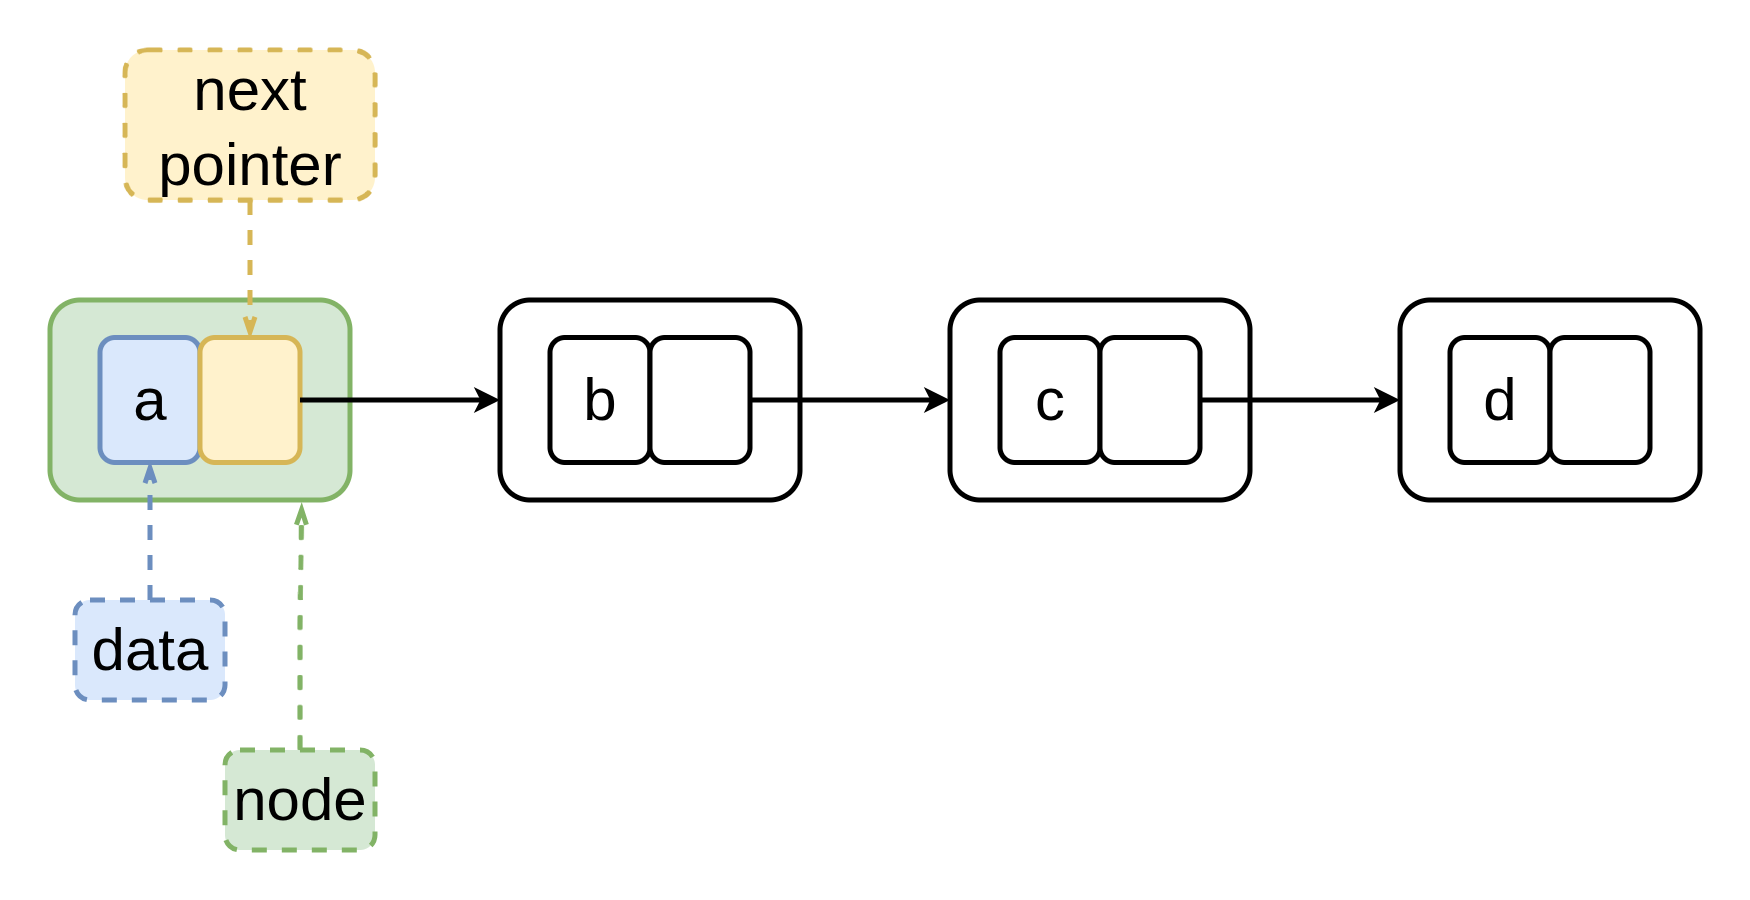
\includegraphics[width=0.8\textwidth]{LLL.png}
\end{center}


\pagebreak
\section{Doubly Linked Lists}
\question{What is unique to Doubly Linked Lists?}

\begin{ansblock}
Doubly Linked Lists have two link directions, next and previous.
\end{ansblock}

\question{Draw a simple 3 element DLL. Label its parts.}

\begin{center}
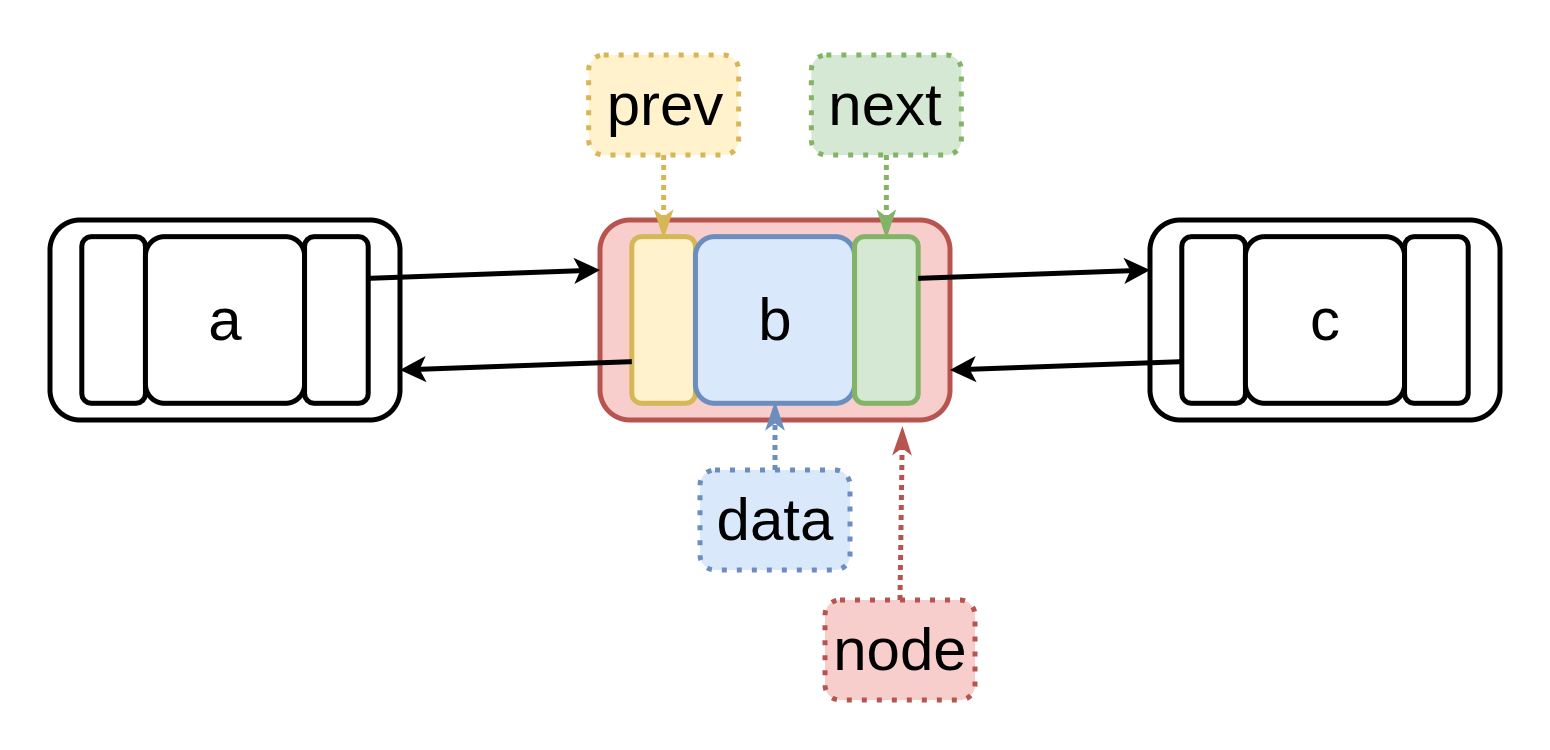
\includegraphics[width=0.8\textwidth]{DLL.png}
\end{center}

\question{What are the three \textit{main} unique cases for removal in a
DLL? Describe the removal process for each case, in plain english.}

\begin{ansblock}
The three \emph{main} cases are:
\begin{enumerate}
    \item Remove head. There are no previous elements to the node being
    removed, so head must be updated after removal. Its next neighbor must be
    updated too.
    \item Remove in the middle of the list. It has two neighbors, that must
    both be updated.
    \item Remove the tail. Its previous neighbor must be updated.
\end{enumerate}

There are also two minor cases, which are trivial. A list with no elements, and
a list with one element.
\end{ansblock}

\pagebreak
\section{Circularly Linked Lists}
\question{What is unique to Circularly Linked Lists?}

\begin{ansblock}
A Circularly Linked List has no distinct end. It wraps back around to the
beginning, typically implemented by keeping track of the last node, with a
\texttt{rear} pointer.
\end{ansblock}

\question{Draw a 5 element CLL. Label its parts.}

\begin{center}
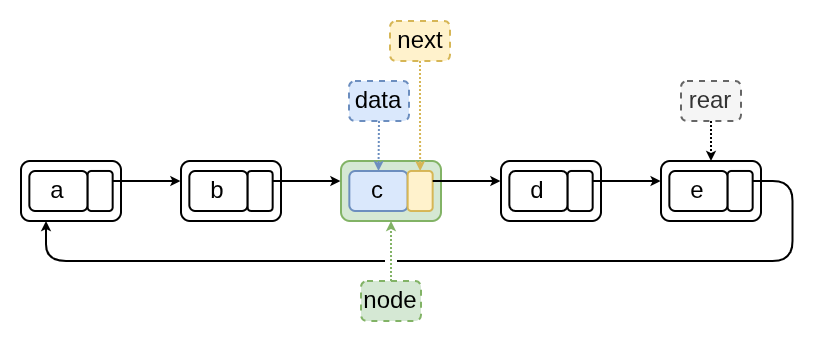
\includegraphics[width=0.8\linewidth]{CLL.png}
\end{center}

\question{What is difficult about iterating over a CLL? Describe the
process in english.}

\begin{ansblock}
In other list types, there is a distinct, separate end value. In C++, this is
the \texttt{nullptr}. CLLs do not have this, so if you are performing some
action over each element, like displaying or reading, then--if you stop right
when you get to the rear--you miss operating on the last element. You need to
account for this in all iterations over a CLL.
\end{ansblock}

\end{document}